%!TEX root = ../../dokumentation.tex

For both RESTful \ac{HTTP} and GraphQL, the same initial setup will be used for prototyping.
Naturally, \textit{node.js} serves as the base engine for interacting with the specific implementation (yellow in Figure \ref{img:prototypesynccomm}), whether it is to provide multiple RESTful \ac{API} endpoints or a single GraphQl endpoint.
For the mockup data to be served over either of the communication technologies, \textit{MongoDB} was chosen together with \textit{Mongoose} as a database connector/driver, due to preexisting experience with said tools.

The exemplary use case is an \ac{API}, which provides information about chefs and dishes. The latter are referenced with a \textit{chefsID} to the chef the dish belongs to.
It should be possible for the client to enter new chefs and dishes, modify, update and delete them, as well as to get an overview of all elements stored in the database (brown in Figure \ref{img:prototypesynccomm}).

\begin{figure}[h]
	\centering
	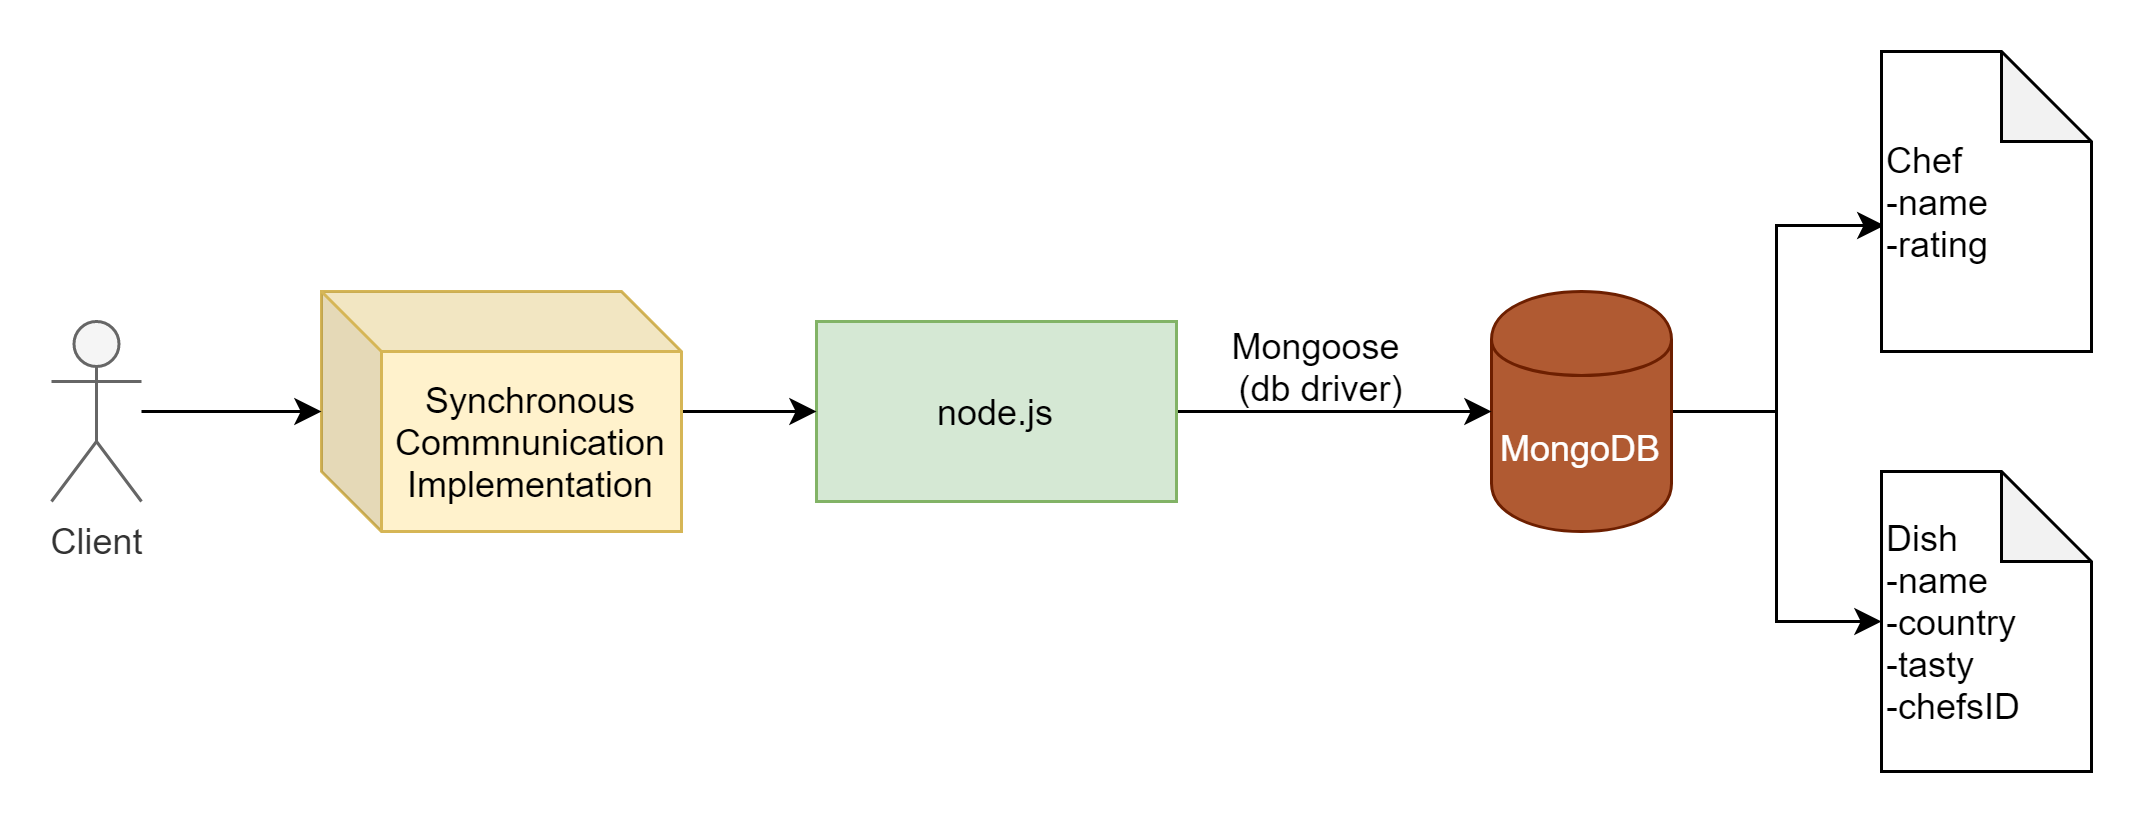
\includegraphics[width=\textwidth, height=0.8\textheight, keepaspectratio]{prototype_sync_comm_overview.png}
	\caption{Prototype setup for synchronous communication}
	\label{img:prototypesynccomm}
\end{figure}

\pagebreak
\textbf{RESTful HTTP}

The prototypic implementation of RESTful \ac{HTTP} endpoints is implemented with the popular server-side web framework \enquote{express.js}.
However, it should be noted that a native implementation of REST is possible with only built in functionalities of \textit{node.js}.
Apart from that, there are also many different middlewares available, such as \textit{sails.js} which make REST modular in its implementation.

The modularity is given because the endpoints are separated from each other.
In the prototypic implementation for example, handler for dishes and chefs are treated individually by their own routes, actions, and call paths (\enquote{http://host/dish} and \enquote{http://host/chef}).
In combination with proxies/gateways the different services can be exchanged, but still be served externally at the same location.

\begin{figure}[h]
	\centering
	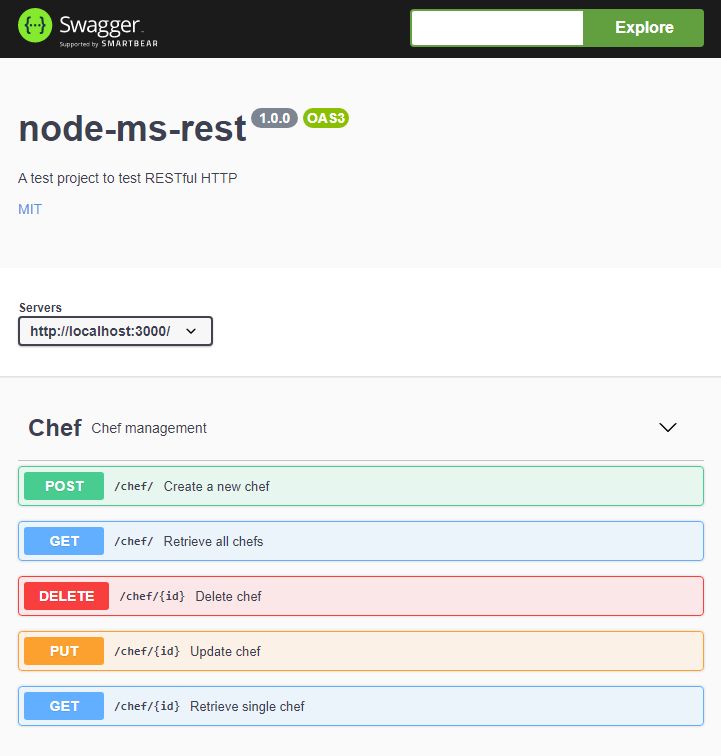
\includegraphics[width=\textwidth, height=0.4\textheight, keepaspectratio]{prototype_rest_swagger.png}
	\caption{Swagger/OpenAPI documentation of the prototypic REST implementation}
	\label{img:prototyperestswagger}
\end{figure}

With \textit{express.js} the learning effort from starting with an existing backend with database connection (cf. Figure \ref{img:prototypesynccomm}) to the first successful REST call was rather low.
This is due to the simplicity that frameworks usually entail.
Although they have a simple syntax, the concept of routing calls and the definition of endpoints must be learned.
As already alluded to in chapter \ref{cha:Technologies:communication:synchronous}, REST itself neither provides strong typing, nor any implementation constraints or specifications to be followed.
While this does offer development flexibility and initial simplicity, the developer and operator must agree on how to access the endpoint.
A basic example of such an agreement is the correct use of \ac{HTTP} verbs as defined in the Richardson Maturity Model (i.e. \textit{DELETE} for deleting resources, \textit{GET} for fetching) \cite{Fowler.2010}.
Consequently, the learning effort increases with the rising application needs, since the introduction of concepts such as hypermedia (i.e. HATEOAS) or versioning may lead to a greater change than with GraphQL.

Since REST itself is only an architectural design introduced by Fielding and later adopted into the \textit{Web Services Architecture (W3C)} and thus subject to the preferences of the developers, there is still no clear definition or \enquote{correct} documentation available on how to implement it \cite{Fielding.15.03.2002}\cite{W3CWorkingGroup.2004}.
Furthermore, there is no clear de facto standard yet, which makes it difficult to define whether an implementation is truly a REST endpoint.
On the other side however, it is common to still benefit from the flexibility, but document the resulting (custom) implementation through specification standards such as \textit{OpenAPI} (or formerly known as \textit{Swagger Specification}).
A screenshot of one of the implemented \textit{Swagger} documentation in the prototype is shown in Figure \ref{img:prototyperestswagger}, where possible operations and the REST endpoints are listed.
Moreover an example call triggered over the web interface of the documentation can be seen in Figure \ref{img:prototyperestcall}.

Apart from concrete \textit{HTTP} client implementations in any programming language, such as \textit{Axios} for JavaScript environments, and the aforementioned documentation tools  there are no other noteworthy extensions for a RESTful \ac{HTTP} service.

\begin{figure}
	\centering
	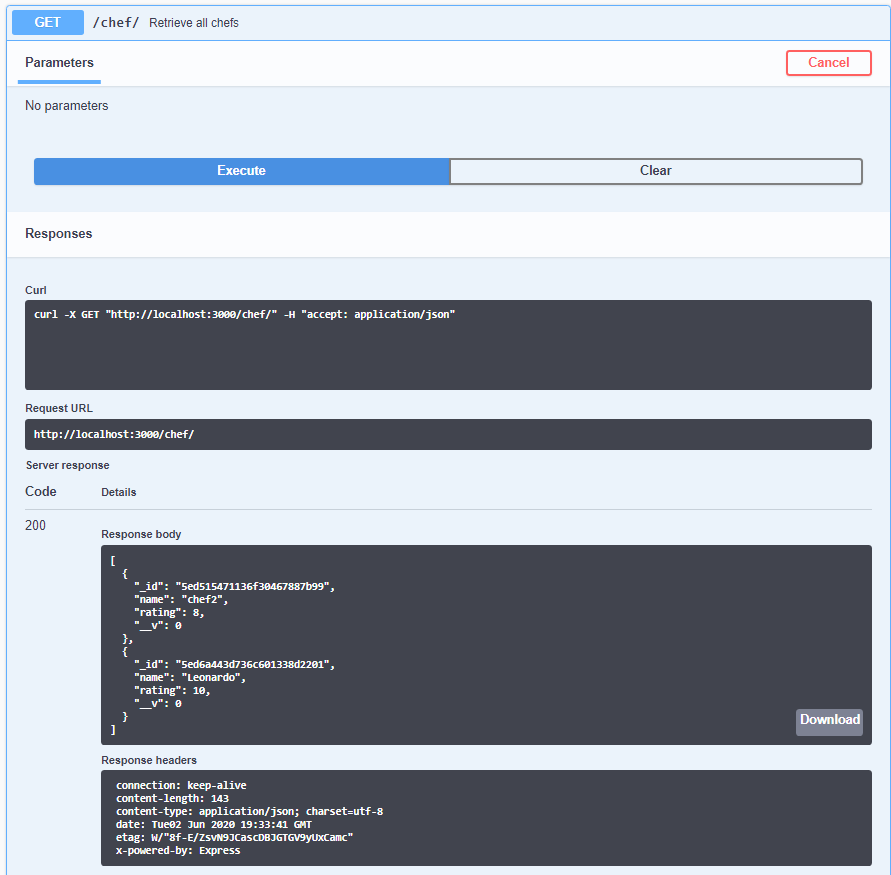
\includegraphics[width=\textwidth, height=0.45\textheight, keepaspectratio]{prototype_rest_swaggercall.png}
	\caption{Exemplary REST call to fetch all chefs using \textit{Swagger}}
	\label{img:prototyperestcall}
\end{figure}

\pagebreak
\textbf{GraphQL}

Similarly to the previous prototype, \enquote{express.js} is used in conjunction with the officially recommended \enquote{express-graphql} connector.
The latter provides options to build the schema for the GraphQL endpoint either with an own language or with JavaScript.
Furthermore, a connector provides an interactive in-browser \ac{IDE} (\enquote{\textit{GraphiQL}}) for executing queries, which includes schema browsing.
As GraphQL is only a specification, other server alternatives to \textit{express-graphql} exist, such as the \textit{Apollo} server.

\begin{figure}
	\centering
	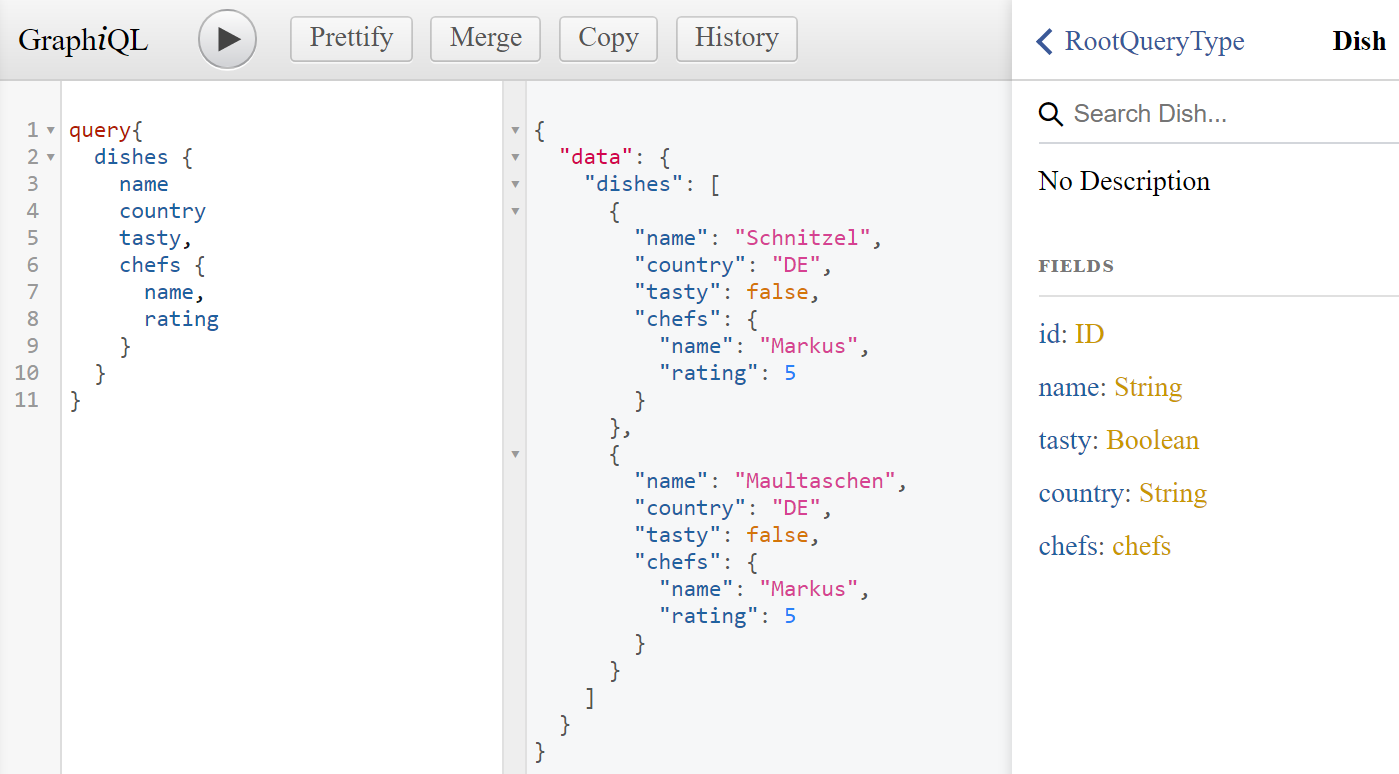
\includegraphics[width=\textwidth, height=0.5\textheight, keepaspectratio]{prototype_graphql_graphiql.png}
	\caption{Exemplary GraphQL call to fetch all dishes and corresponding chefs using \textit{GraphiQL}}
	\label{img:prototypegraphiql}
\end{figure}

For the prototypic implementation, the focus was on implementing a GraphQL \ac{API} handler that accepts queries over a \ac{HTTP} endpoint.
Consequently, any \ac{HTTP} enabled client can access the GraphQL backend without much implementation effort.
However, it should be noted, that for production environments more complex clients, which may include batching, caching and other optimizations, exist and should be used (e.g. \textit{Apollo} client).
With the current implementation, an exemplary query (as shown in Figure \ref{img:prototypegraphiql}) can be executed, either with a \textit{POST} \ac{HTTP} call or by using \textit{GraphiQL}.
As already outlined in chapter \ref{cha:Technologies:communication:synchronous}, although the same database is used as in the previous prototype, GraphQL allows the client to retrieve only the needed information, including nesting (i.e. retrieve attributes from chefs connected to the dish in this example).

Regarding modularity, there is no native support for splitting  a GraphQL instance and its underlying scheme definition, thus providing modularity.
However, for officially referenced toolsets that were not part of this prototype, \enquote{schema stitching} is one way to achieve modularity.
Figure \ref{img:prototypegraphqlproxy} shows how multiple GraphQL servers can be combined with each own database connection and scheme, even together with different RESTful \ac{HTTP} endpoint, allowing the client to submit a query to a single GraphQL endpoint.

The extension \textit{graphql-tools} for stitching is only one of many available extensions for GraphQL.
Besides the plethora of available client and server implementations for each programming language, third party libraries and tools are also available.
Examples are a content management system (\textit{graphcms} or \textit{tipe}), visualization tools (\textit{graphql voyager}), documentation platforms \textit{GraphQL Docs} and the popular fullstack platform \textit{Apollo}.
Consequently, although GraphQL is not as simple as a RESTful \ac{API}, its widespread support makes it very flexible.

\begin{figure}[h]
	\centering
	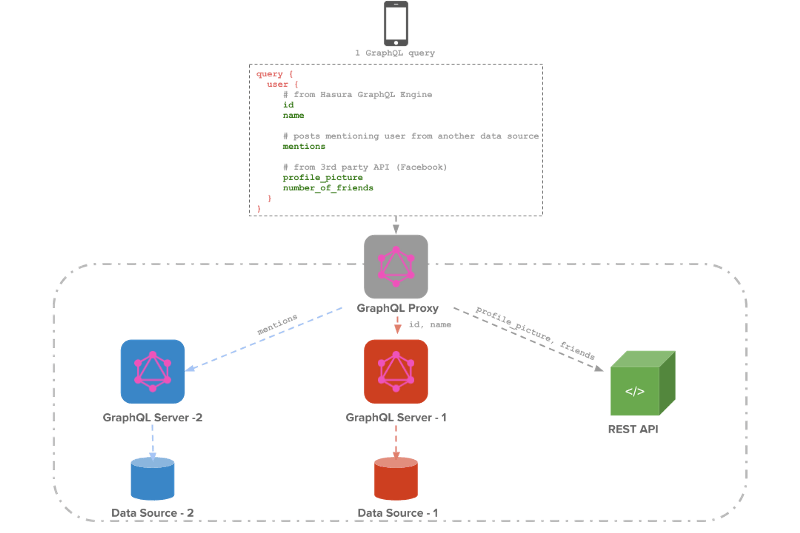
\includegraphics[width=\textwidth, height=0.3\textheight, keepaspectratio]{prototype_graphql_proxy.png}
	\caption{Combining different data sources - schema stitching using \textit{graphql-tools} extension \cite{Wawhal.2018}}
	\label{img:prototypegraphqlproxy}
\end{figure}

GraphQL itself mostly provides reference implementations that are officially documented but are often superceded by third party implementations.
All concepts, scheme language definition and best practices are documented extensively on the official website.
This includes the \ac{API} reference for reference implementations (in this case \textit{graphql-js}), on which additional libraries, such as the one used in the prototype are built upon (\textit{express-graphql}).
On the contrary, as third party implementations are often used due to their ease of use and simplification, the practical usage of GraphQL may be bound to external documentation, making a general statement about the level of documentation of GraphQL difficult.

Nevertheless, the documentation is helpful in learning how to use GraphQL.
As the schema language, typing and the general concept of queries and mutations must be learned to use GraphQL, the learning effort is to be rated as moderate.
While documentation is available, the learning curve may be steep at first due to the new concepts, especially when never having dealt with graph-based databases before.

\textbf{Conclusion}

As expected, REST is easier to implement due to its loose specification, while GraphQL presents itself as a well thought-out and exhaustive framework with many features, but which requires learning initial concepts.
The synchronous communication in the exemplary LAN party application will mostly be found in communication of the web-based frontend with the backend services instead of the inter-service communication.
This circumstance does not exclude the possibility of using GraphQL or REST in the backend.
However, in this application, the publish-subscribe pattern with asynchronous communication may be suited better, which is why the evaluation focuses on the frontend communication.

For the final implementation, REST is selected because of the lower learning effort and the broad and simple compatibility.
Especially for the client side, which is a web browser in this case, it is easier to implement a connection to the REST \ac{API}, than with GraphQL, which often needs more than a simple \textit{POST} request, but rather client tooling for maintainability and performance.
Although the clients in this use case are performant enough to be more than \textit{thin clients} and could handle more complex operations, REST is more sensible here.
There are very few cases where data needs to be retrieved, manipulated or actions need to be triggered which GraphQL would perform better.
Such a possible feature would be, for example,  browsing for teams in the scoreboard and displaying recent matches of the team.
Although this would be a feature where GraphQL would excel, other, less complex features would have to be built with the same amount of complexity compared to REST.

Nevertheless, GraphQL, with its contract-driven design, introspection, and thus consistent endpoint and schema declaration, clearly overshadows REST for moderate and complex operations.
However, in the context of the LAN party application, the effort needed to achieve the aforementioned benefits is unjustifiable compared to the actual, relatively simple needs covered by REST.
Finally, however, as GraphQL can and is often used on top of existing (cf. chapter \ref{cha:Technologies:communication:graphql}) REST \acp{API}, an extension at a more developed stage of the LAN party application should be taken into consideration, in order to benefit from GraphQL's features, while providing REST alongside in a hybrid approach.
